\newpage
\section{Introduction}
When computing a result over a data type, a small change would lead to completely recomputing the result. Parts of the recomputation give the same results as the previous computation. By keeping track of the intermediate results and reusing the results when the input is the same, fewer computations have to be performed. 

An example of computing a result over a data type is computing the \textbf{maximum path sum} over a binary tree. Given a \inlinehaskell{BinTree}, starting at the root node, find a path from the root node to the leaves that leads to the maximum total.

The implementation of the computation is done in \texttt{Haskell}. And the definition of the binary tree and example is:
\begin{haskell}
data BinTree = Leaf Int
             | Node BinTree Int BinTree 
\end{haskell}

\begin{haskell}
exampleTree :: BinTree    
exampleTree = Node (Node (Leaf 8) 7 (Leaf 9)) 3 (Node (Leaf 5) 4 (Leaf 2))
\end{haskell}

\begin{figure}[H]
    \centering
    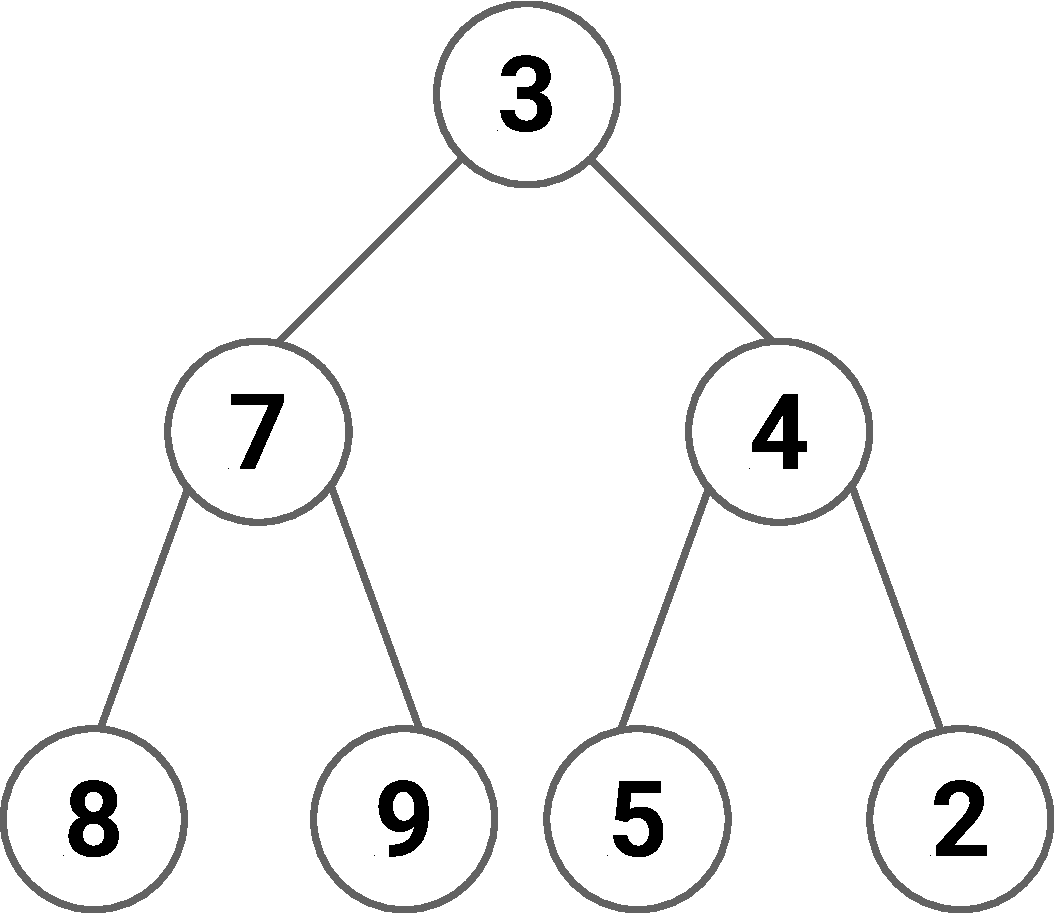
\includegraphics[width=.4\textwidth]{Tree.pdf}
    \caption{Graphic visualization of the \inlinehaskell{exampleTree}}
\end{figure}

An implementation of computing the max path sum over data type \inlinehaskell{BinTree} is and has a complexity of $\mathcal{O}(N)$.
\begin{haskell}
maxPathSum :: BinTree -> Int
maxPathSum (Leaf x)     = x
maxPathSum (Node l x r) = x + max (maxPathSum l, maxPathSum r)
\end{haskell}

\newpage
And computing the max path sum over the \inlinehaskell{exampleTree} results in 19.

\begin{figure}[H]
\begin{minipage}[c]{0.35\textwidth}
\begin{haskell}
maxPathSum exampleTree !$\equiv$! 19
\end{haskell}
\end{minipage}
\hspace{0.1\textwidth}
\begin{minipage}[c]{0.55\textwidth}
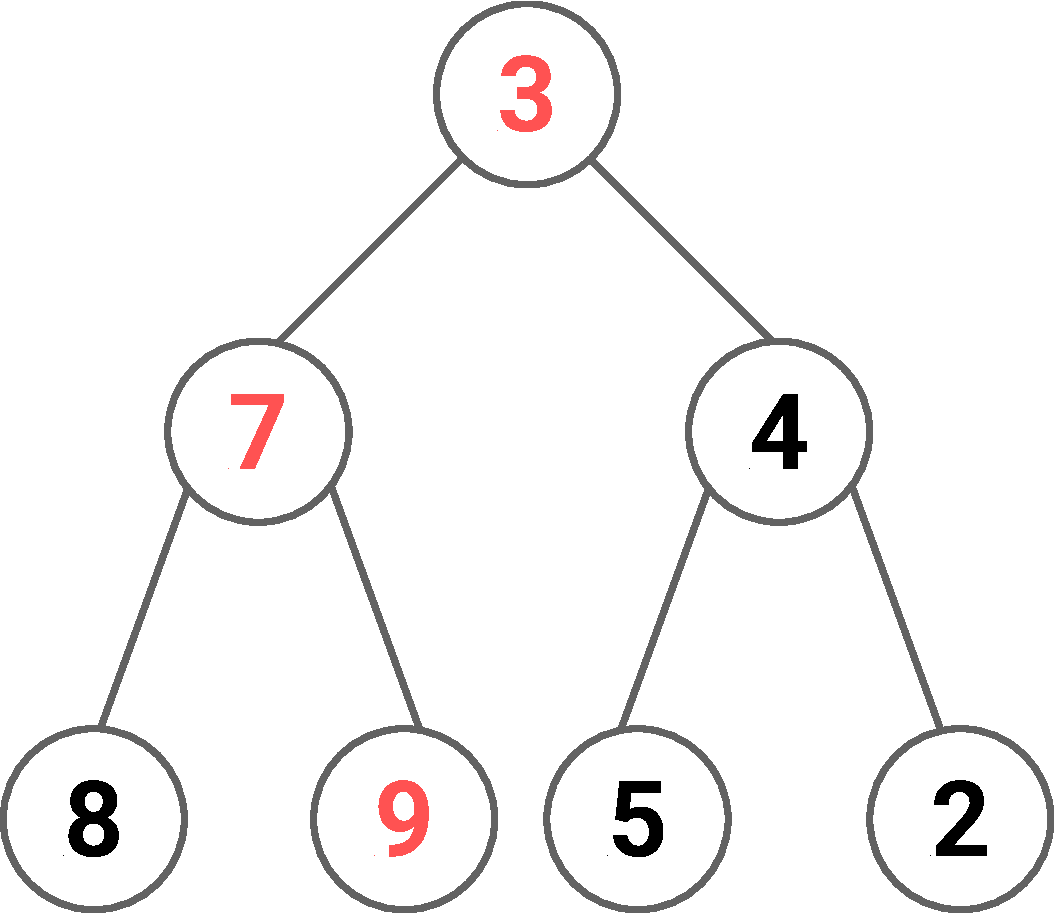
\includegraphics[width=0.7\textwidth]{SolvedTree.pdf}
\end{minipage}
\end{figure}

\todo[inline]{Add function complexities to the explanation}
To reduce the number of recomputations, first, we need to compare the structure of the data type for equality. When comparing the data type structure for equality, if they are equal, the previously computed result can be reused. Otherwise, the result needs to be recomputed. To compare the structure of the data type in constant time, we introduce the use of hash functions. Generating a hash every time a comparison takes place would be inefficient because part of the structure does not change, which leads to the same hash. Thus, every substructure in the data type stores the hash of its substructure. 

In the example, a new data type is introduced: the \inlinehaskell{MerkleTree}. This data type is the same as the \inlinehaskell{BinTree}, but the constructors also contain a \inlinehaskell{Hash}. To create a \inlinehaskell{MerkleTree}, we traverse through a \inlinehaskell{BinTree} and hash the structure and store it. Creating a \inlinehaskell{MerkleTree} has a time complexity of $\mathcal{O}(N)$.

\begin{haskell}
data MerkleTree = LeafH Hash Int
                | NodeH Hash MerkleTree Int MerkleTree

merkle :: BinTree -> MerkleTree
merkle (Leaf x)     = LeafH (hash ["Leaf", x]) x
merkle (Node l x r) = NodeH (hash ["Node", x, hl, hr]) l' x r'
  where
    hl = getHash l'
    hr = getHash r'
    l' = merkle l
    r' = merkle r
\end{haskell}

\begin{figure}[H]
    \centering
    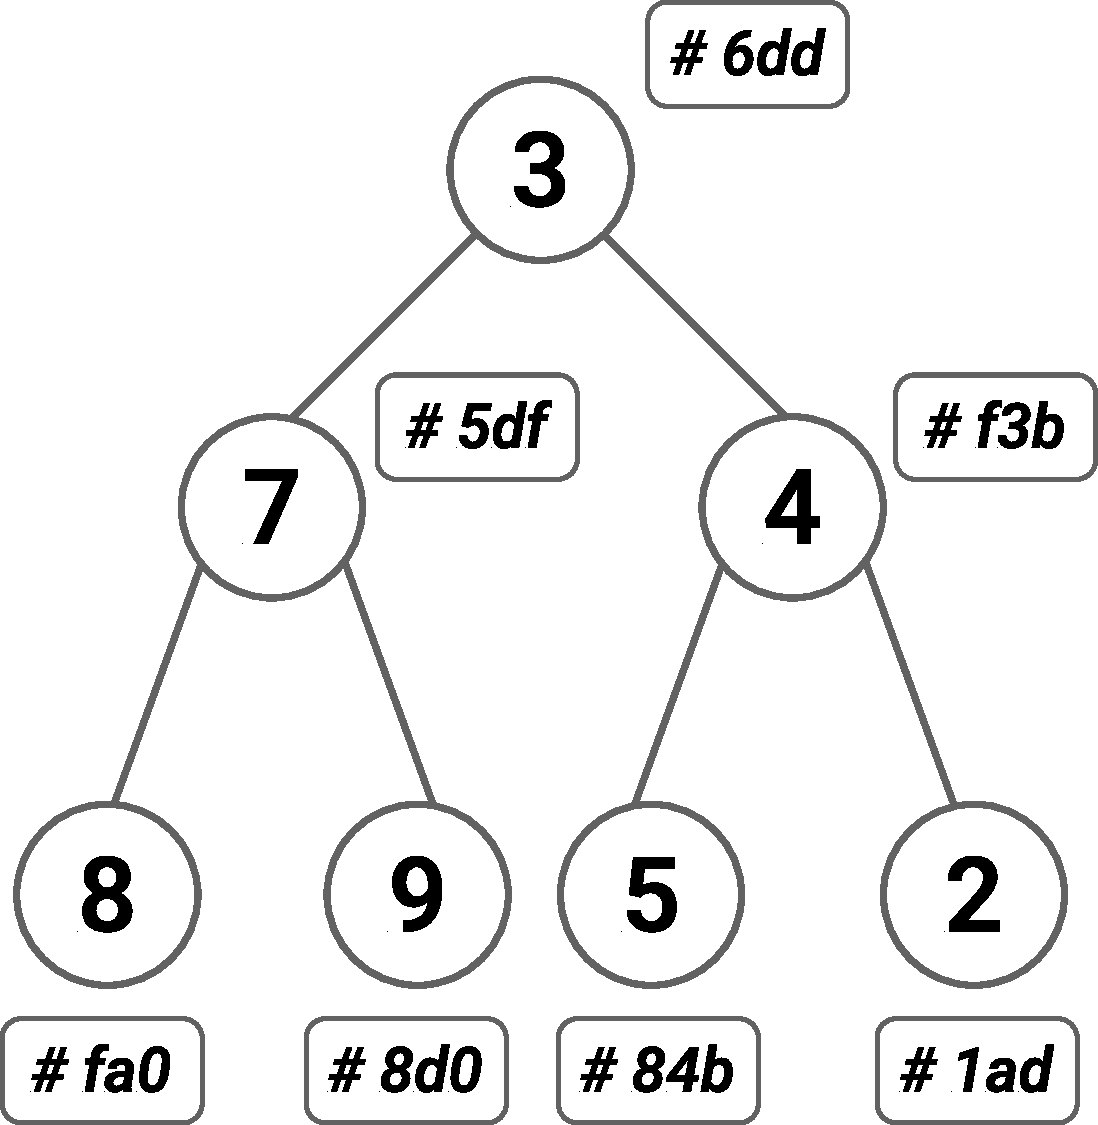
\includegraphics[width=.4\textwidth]{MerkleTree.pdf}
    \caption{The \inlinehaskell{MerkleTree} of \inlinehaskell{exampleTree}}
\end{figure}

To compute the max path sum and its intermediate results, we can use the precomputed hashes of the \inlinehaskell{MerkleTree} to efficiently generate a \inlinehaskell{Map Hash Int}. The complexity of computing the max path sum and the intermediate results is $\mathcal{O}(N)$.   

The example implementation of computing the max path sum and its intermediate results can be seen below. However this implementation uses a \texttt{union} (\inlinehaskell{<>}) to combine the \inlinehaskell{Map}'s which has a complexity of $\mathcal{O}(m*log(n/m + 1)), m <= n$. This can be implemented more efficiently by giving the \inlinehaskell{Map} to the left side and then to the right side of the Tree, which makes it a constant operation. Except, this would make the code more complex. 

\begin{haskell}
maxPathSumInc :: MerkleTree -> (Int, Map Hash Int)    
maxPathSumInc (LeafH h x)     = (x, insert h x empty)
maxPathSumInc (NodeH h l x r) = (y, insert h y (ml <> mr))  
  where
    y = x + max (xl, xr)
    (xl, ml) = maxPathSumInc l
    (xr, mr) = maxPathSumInc r
\end{haskell}
\vspace{15pt}
\begin{figure}[H]
    \begin{minipage}[c]{0.55\textwidth}
        \centering
        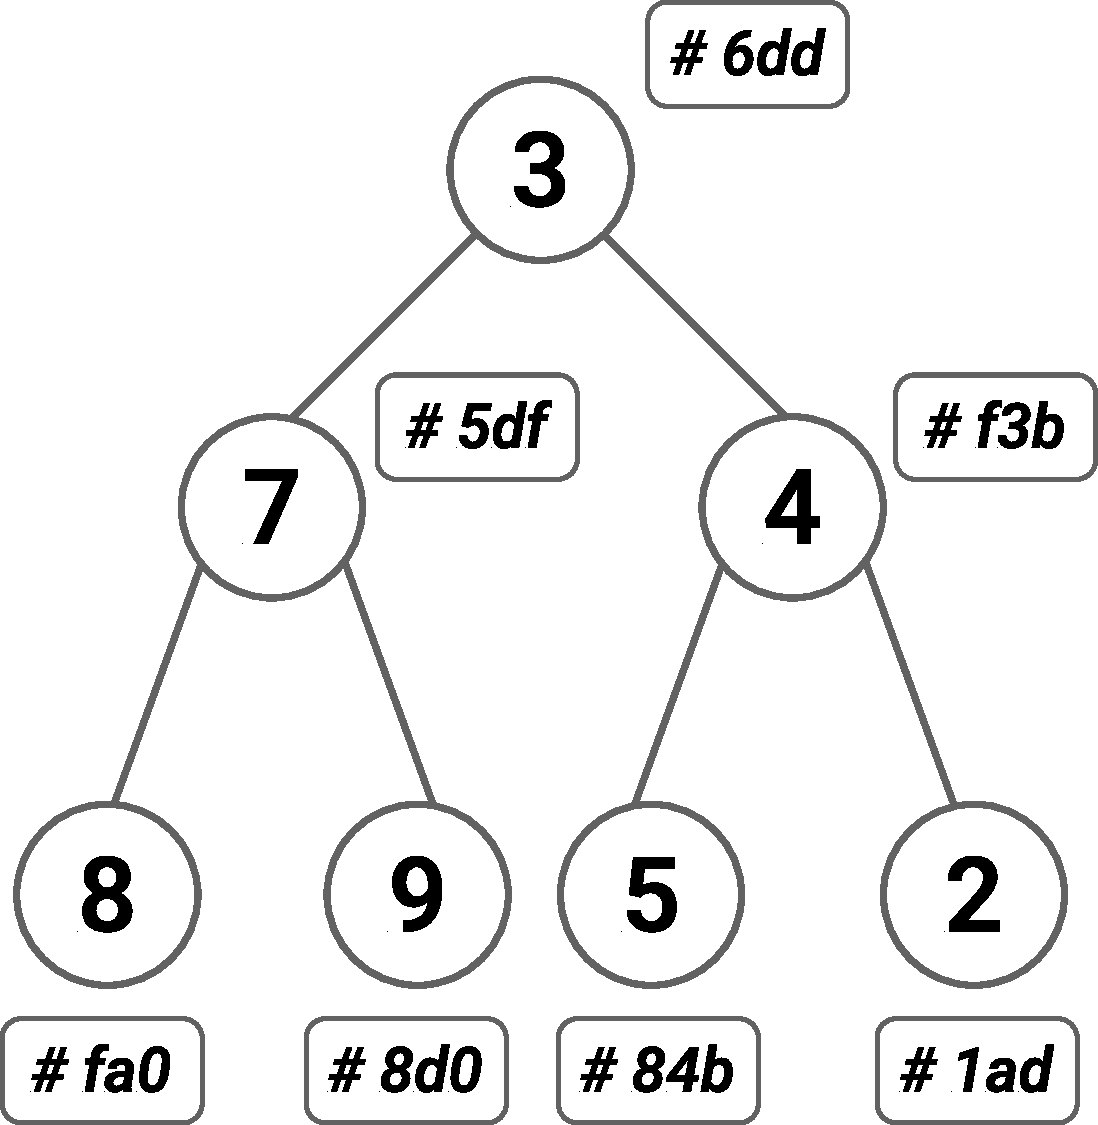
\includegraphics[width=.7\textwidth]{MerkleTree.pdf}
    \end{minipage}
    \hspace{0.1\textwidth}
    \begin{minipage}[c]{0.35\textwidth}
        \centering
        \begin{tabular}{|l|r|}
            \hline
            \textbf{Hash Nodes} & \textbf{Max Sum} \\
            \hline
            \# 6dd & 19 \\
            \hline
            \# 5df & 16 \\
            \hline
            \# fa0 & 8 \\
            \hline
            \# 8d0 & 9 \\
            \hline
            \# f3b & 9 \\
            \hline
            \# 84b & 5 \\
            \hline
            \# 1ad & 2 \\
            \hline
        \end{tabular}
    \end{minipage}
    \caption{The \inlinehaskell{MerkleTree} with intermediate results}    
\end{figure}

When there is a change in the \inlinehaskell{BinTree}, only the hashes of the change itself and its parents need to be recomputed. The recomputation of the hash has a time complexity of $\mathcal{O}(M \log{N})$ where $M$ is the number of changed nodes.

\begin{figure}[H]
    \centering
    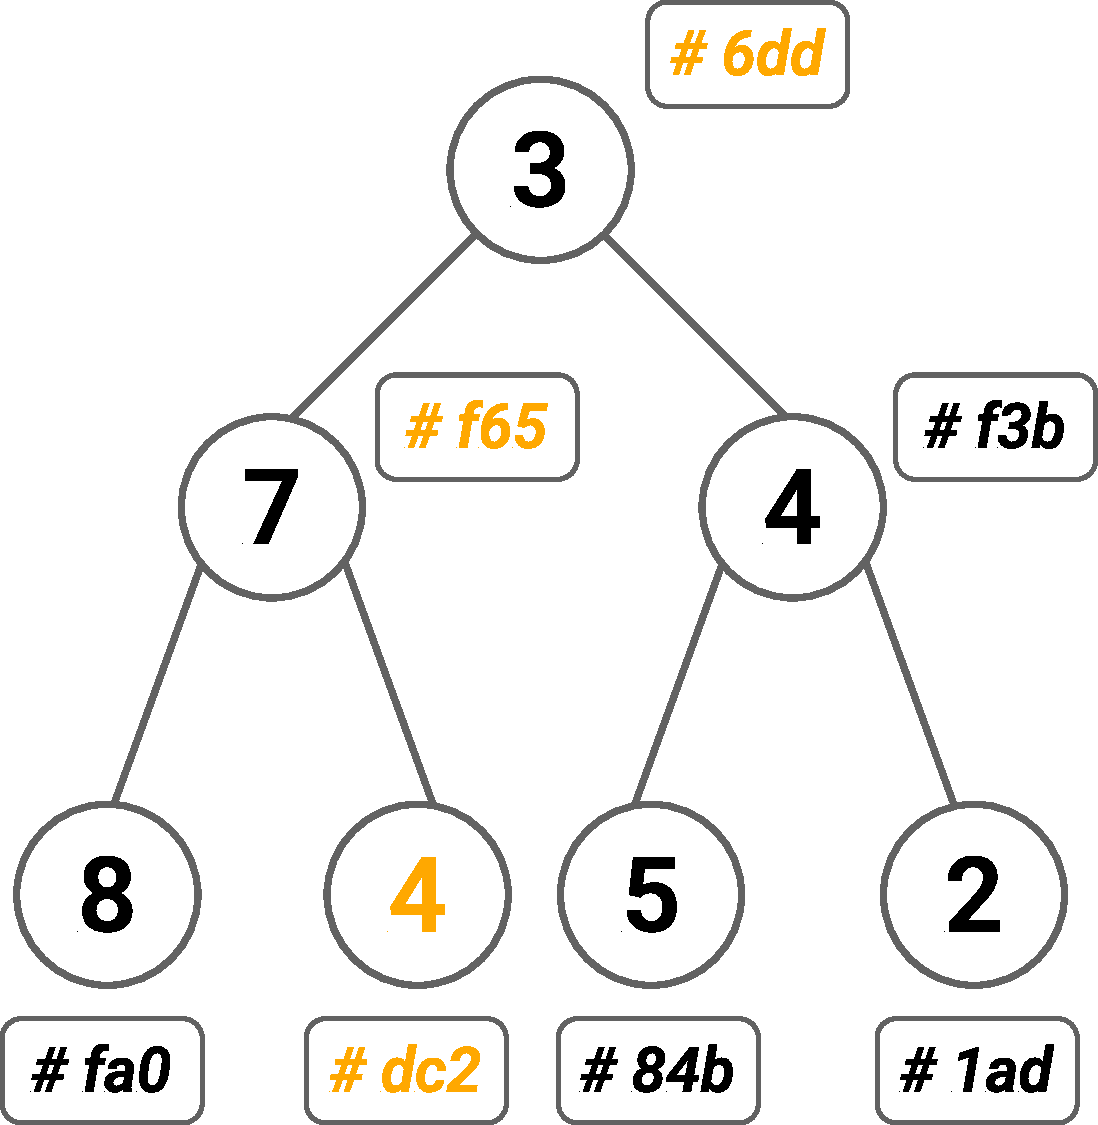
\includegraphics[width=.33\textwidth]{ChangedMerkleTree.pdf}
    \caption{Changed Merkle Tree}
\end{figure}

Then to compute the max path sum over the Changed Tree, the previously computed \texttt{Map} can be used to reduce the amount of recomputation.  

\begin{haskell}
maxPathSumMap :: Map Hash Int -> MerkleTree -> (Int, Map Hash Int)
maxPathSumMap m (LeafH h x) = case lookup m h of
  Just y  -> (y, m)
  Nothing -> (x, insert h x m)
maxPathSumMap m (NodeH h l x r) = case lookup m h of
  Just y  -> (y, m)
  Nothing -> (y, insert h y (ml <> mr))
    where
      y = x + max (xl, xr)
      (xl, ml) = maxPathSumMap m l
      (xr, mr) = maxPathSumMap m r  
\end{haskell}

In this paper, an implementation of storing the intermediate results is presented, supporting generic data types. That means the developer only needs to implement the max path sum functionality and the intermediate results are automatically stored.

\begin{table}[H]
    \centering
    \begin{tabular}{|l|r|r|}
        \hline
        \textbf{Function} & \textbf{Average} & \textbf{Upperbound} \\
        \hline
        \inlinehaskell{merkle} & $\Theta(N)$ & $\mathcal{O}(N)$ \\
        \hline
        \inlinehaskell{maxPathSumInc} & $\Theta(N)$ & $\mathcal{O}(N)$ \\
        \hline
        Change Merkle Tree & $\Theta(M \log{N})$  & $\mathcal{O}(N)$ \\
        \hline
        \inlinehaskell{maxPathSumMap} & $\Theta(M \log{N})$  & $\mathcal{O}(N)$ \\
        \hline
    \end{tabular}
\end{table}

\begin{table}[H]
    \centering
    \begin{tabular}{|l|r|r|}
        \hline
        \textbf{Function} & \textbf{Average} & \textbf{Upperbound} \\
        \hline
        \inlinehaskell{maxPathSum} & $\mathcal{O}(N)$ & $\mathcal{O}(N)$ \\
        \hline
    \end{tabular}
\end{table}

\newpage
\subsection{Contributions}
\begin{enumerate}[label={(\Alph*)}]
    \item A library needs to be implemented which contains the generic \texttt{merkle}, \texttt{cataMerkle} and \texttt{cataMerkleWithMap} functions
\end{enumerate}

\subsection{Research Questions}
Using the previously mentioned library, there is a multitude of questions to be answered:
\begin{enumerate}[label={(\Alph*)}]
    \item What parameters can be tweaked to have the best ratio of performance and memory usage?
    \item What type of equivalence is needed to reuse the incremental computation?
    \item What type of data structures are the best for storing the incremental computation?
    \item Could the library be used to perform static analysis in a more performant manner?
\end{enumerate}